\documentclass[12pt]{article}

\usepackage[utf8]{inputenc}
\usepackage[T1]{fontenc}
\usepackage{lmodern}
\usepackage[margin=1in]{geometry}
\usepackage{amsmath,amsthm,amssymb}
\usepackage{listings}
\usepackage{xcolor}
\usepackage{booktabs}
\usepackage{graphicx}
\usepackage{tikz}
\usetikzlibrary{arrows.meta,positioning,calc}
\usepackage{array}
\usepackage{makecell}
\usepackage{float}
\usepackage{parskip}
\usepackage[hidelinks]{hyperref}

%% Theorem environments
\newtheorem{definition}{Definition}
\newtheorem{proposition}{Proposition}
%% Inline code
\newcommand{\code}[1]{\texttt{#1}}

%% Java listings
\definecolor{codegray}{gray}{0.45}
\definecolor{codeblue}{rgb}{0.13,0.29,0.53}
\definecolor{codebg}{rgb}{0.97,0.97,0.97}
\lstdefinestyle{java}{
  language=Java,
  basicstyle=\small\ttfamily,
  keywordstyle=\color{codeblue}\bfseries,
  commentstyle=\color{codegray}\itshape,
  stringstyle=\color{codegray},
  backgroundcolor=\color{codebg},
  frame=single,
  framesep=4pt,
  rulecolor=\color{black!15},
  xleftmargin=6pt,
  xrightmargin=6pt,
  breaklines=true,
  breakatwhitespace=true,
  showstringspaces=false,
  tabsize=2,
  numbers=none,
  morekeywords={abstract,implements,extends,interface,class,new,return,
                public,private,protected,static,final,void,String,boolean,
                int,Object,Override,System,out,println},
}
\lstset{style=java}

%% Kotlin listings
\lstdefinestyle{kotlin}{
  language=,
  basicstyle=\small\ttfamily,
  keywordstyle=\color{codeblue}\bfseries,
  commentstyle=\color{codegray}\itshape,
  stringstyle=\color{codegray},
  backgroundcolor=\color{codebg},
  frame=single,
  framesep=4pt,
  rulecolor=\color{black!15},
  xleftmargin=6pt,
  xrightmargin=6pt,
  breaklines=true,
  breakatwhitespace=true,
  showstringspaces=false,
  tabsize=2,
  numbers=none,
  morekeywords={fun,val,var,class,interface,override,by,abstract,open,
                private,public,protected,String,Unit,Any,return,if,else},
}


\begin{document}

\title{Interface-Scoped Dispatch:\\
Object Composition with O(1) Self-Calls}
\author{R. Scott McKinney\\
\textit{scott@manifold.systems}}
\date{}
\maketitle

\begin{abstract}
Object composition forces a trade under static typing: independent
components, or correct self-call dispatch. Forwarding-based tools supply independent components, but a component's
self-calls resolve within the component, not the composite. Trait and
mixin composition preserves self-call dispatch at the expense of independent
components. Neither delivers both. Achieving both at the cost of ordinary
dispatch, in a statically-typed language, is the open problem.

We present \emph{Parts}, realized as a compiler plugin for Java~8--26.
The enabling mechanism is \emph{interface-scoped dispatch} (ISD): composite
identity is assigned per interface rather than per object, so self-calls route
through the correct composite in arbitrary DAG compositions. The dispatch cost is
one array-indexed load plus standard \texttt{invokeinterface}, structurally
equivalent to vtable dispatch and empirically corroborated. Parts supports
DAG composition with multiple composite roots per component, resolves diamond
ambiguity statically, and introduces composite-scoped encapsulation.
\end{abstract}

\tableofcontents

%% ─────────────────────────────────────────────────────────────────────────────
\section{Introduction}
%% ─────────────────────────────────────────────────────────────────────────────

Object composition is the standard prescription for avoiding implementation
inheritance~\cite{gamma1994}. Two properties make it a genuine replacement:
\emph{independent components}---unrestricted late-bound objects fixed at
construction---and correct self-call dispatch through the composite.
Static typing is what makes the two hard to combine: dynamically-typed object
models have had both for decades, yet no statically-typed language
provides them together at the cost of ordinary dispatch.

Forwarding-based composition (Kotlin \code{by}~\cite{kotlin}, Lombok
\code{@Delegate}~\cite{lombok}) supplies independent components but does not
support open recursion: a component's self-calls resolve within the component
because the composite is never on the dispatch path. This is
the Self problem~\cite{lieberman1986,self1987}, identified in 1986.

Trait composition (Scala \code{with}~\cite{odersky2005},
mixins~\cite{bracha1990}) inverts the trade. Self-calls dispatch through
\code{this} in the linearized class, so composite overrides are visible. But
traits are fused into the class hierarchy at compile time, not supplied as
runtime objects. Components cannot be constructed independently and passed in;
composition is static.

\emph{Parts} provides both. \code{@part} marks a class as a component; \code{@link} marks a field through which a composite
delegates one or more interfaces to that component. Components are independent
objects supplied at construction time. When a composite is constructed, a
compiler plugin wires composite identity into each component, so self-calls in
the component dispatch through the composite. The enabling mechanism is
\emph{interface-scoped dispatch} (ISD): assigning composite identity per
interface rather than per object enables correct self-call dispatch in all Parts compositions.

The core contributions are:

\begin{itemize}
  \item \textbf{Parts}: a model for object composition in which
        components are independent runtime objects, self-calls dispatch through
        the composite, and interface contracts are statically enforced.
        The model is defined over a standard typed object model with a central
        dispatch invariant (Proposition~\ref{prop:dispatch}) and
        composite-scoped encapsulation (\code{@internal}).
  \item \textbf{Interface-scoped dispatch (ISD)}: the mechanism that assigns
        composite identity per interface rather than per object, enabling
        correct self-call dispatch in Parts compositions, including partial
        delegation (where a composite claims a proper subset of a component's
        interfaces) and arbitrary DAG compositions.
  \item \textbf{A practical implementation}: a compiler plugin for
        Java 8--26 realizing the model at O(1) dispatch cost, with open-source
        release~\cite{mckinney2026} and IDE integration.
\end{itemize}

%% ─────────────────────────────────────────────────────────────────────────────
\section{Overview}
%% ─────────────────────────────────────────────────────────────────────────────

Consider a minimal example that shows \code{@part} and \code{@link} working in a concrete single-rooted composite.

\begin{lstlisting}
interface Formatter {
    String prefix();
    String format(String msg);
}

@part class LogFormatter implements Formatter {
    public String prefix() { return "INFO"; }
    public String format(String msg) { return "[" + prefix() + "] " + msg; }
}

class AppFormatter implements Formatter {
    @link Formatter fmt;
    AppFormatter(Formatter f) { this.fmt = f; }
    @Override public String prefix() { return "APP"; }
}

new AppFormatter(new LogFormatter()).format("started"); // "[APP] started"
\end{lstlisting}

When \code{AppFormatter} is constructed, the compiler wires
\code{LogFormatter}'s composite identity for \code{Formatter} to
\code{AppFormatter}. A call to \code{format("started")} dispatches to
\code{LogFormatter.format()}, and the self-call \code{prefix()} within
\code{format()} dispatches back through \code{AppFormatter}, invoking
\code{AppFormatter.prefix()}, not \code{LogFormatter.prefix()}.

Because the \code{@link} field accepts any \code{Formatter} at construction
time, the component is a real runtime object, not fused into the class
hierarchy. A different \code{Formatter} implementation can be substituted
without changing \code{AppFormatter}.

Interface contracts are enforced at compile time: the \code{@link} field has
type \code{Formatter}, and the compiler verifies that \code{AppFormatter}
implements the delegated interface. Component identity may not escape the
composite dispatch path: passing or assigning \code{this} as the concrete
\code{@part} type is a compile error; interface types are required.

This example is single-rooted: \code{AppFormatter} is the sole composite
for \code{LogFormatter}, and one composite identity suffices. The following
section exposes the limit of the single-identity model and the per-interface
generalization that resolves it.

%% ─────────────────────────────────────────────────────────────────────────────
\section{The Model}
\label{sec:model}
%% ─────────────────────────────────────────────────────────────────────────────

\subsection*{Motivating example}

The following example shows a component with multiple interface roots, each
requiring a distinct composite identity. \code{Track} implements both
\code{Streamable} and \code{Classifiable}; in the composed graph,
\code{Streamable} is rooted at \code{Playlist} and \code{Classifiable} is
rooted at \code{Library}. From the same \code{Track} instance, a self-call to
\code{codec()} must route through \code{Playlist} and a self-call to
\code{genre()} through \code{Library}. A single identity slot cannot hold
both. A per-interface identity array---\code{\$selves[IDX\_I]}, at the compile-time
index \code{IDX\_I} assigned to interface~$I$, holds the composite identity for
$I$ independently of every other interface---provides exactly one root per
interface.
Figures~\ref{fig:dag-diagram} and~\ref{fig:dag-listing} show the structure.

\begin{figure}[H]
\centering
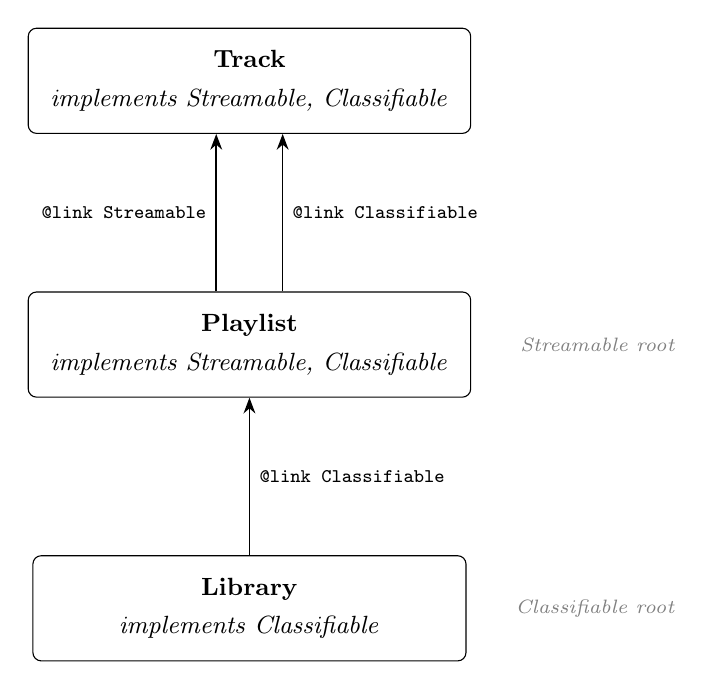
\begin{tikzpicture}[
  cls/.style={
    draw, rectangle, rounded corners=3pt,
    minimum width=5.5cm, inner sep=8pt,
    align=center, font=\small
  },
  lnk/.style={->, >=Stealth, semithick},
]
\node[cls] (wp)
  {\textbf{Track}\\[3pt]
   \textit{implements Streamable, Classifiable}};

\node[cls, below=2cm of wp] (lw)
  {\textbf{Playlist}\\[3pt]
   \textit{implements Streamable, Classifiable}};

\node[cls, below=2cm of lw] (app)
  {\textbf{Library}\\[3pt]
   \textit{implements Classifiable}};

%% Playlist @link -> Track
\draw[lnk] ([xshift=-12pt]lw.north)
  -- node[left,  font=\scriptsize\ttfamily] {@link Streamable}
  ([xshift=-12pt]wp.south);
\draw[lnk] ([xshift=12pt]lw.north)
  -- node[right, font=\scriptsize\ttfamily] {@link Classifiable}
  ([xshift=12pt]wp.south);

%% Library @link -> Playlist
\draw[lnk] (app.north)
  -- node[right, font=\scriptsize\ttfamily] {@link Classifiable}
  (lw.south);

%% Dispatch root annotations
\node[font=\scriptsize\itshape, text=gray, right=0.5cm of lw, anchor=west]
  {Streamable root};
\node[font=\scriptsize\itshape, text=gray, right=0.5cm of app, anchor=west]
  {Classifiable root};
\end{tikzpicture}
\caption{DAG composition structure. Arrows show \code{@link} fields labeled
by the delegated interface. \code{Playlist} is the root for
\code{Streamable} dispatch; \code{Library} is the root for \code{Classifiable} dispatch.}
\label{fig:dag-diagram}
\end{figure}

\begin{figure}[H]
\begin{lstlisting}
interface Streamable {
    String codec();
    void stream(String audio);
}

interface Classifiable {
    String genre();
    String classify(String title);
}

@part class Track implements Streamable, Classifiable {
  public String codec()  { return "wav"; }
  public String genre()  { return "unknown"; }
  public void stream(String audio) { System.out.println("[" + codec() + "] " + audio); }
  public String classify(String title) {
    stream("indexing: " + title);   // Streamable dispatch
    return genre() + ":" + title;   // Classifiable dispatch
  }
}

@part class Playlist implements Streamable, Classifiable {
  @link Streamable   streamable;
  @link Classifiable classifiable;
  Playlist(Track t) { this.streamable = t; this.classifiable = t; }
  @Override public String codec() { return "mp3"; }
}

class Library implements Classifiable {
  @link Classifiable classifiable;
  Library(Classifiable c) { this.classifiable = c; }
  @Override public String genre() { return "jazz"; }
}

Playlist playlist = new Playlist(new Track());
Library library   = new Library(playlist);
String result = library.classify("Autumn Leaves");
out.println(result);
// Streamable dispatch rooted at Playlist  ->  codec()  -> "mp3"
// Classifiable dispatch rooted at Library ->  genre()  -> "jazz"
// prints:  "[mp3] indexing: Autumn Leaves"
// returns: "jazz:Autumn Leaves"
\end{lstlisting}
\caption{DAG composition with multiple composite roots per component.
\code{Track} carries distinct composite identities for \code{Streamable}
(rooted at \code{Playlist}) and \code{Classifiable} (rooted at \code{Library}).}
\label{fig:dag-listing}
\end{figure}

\subsection*{Definitions}

We define Parts over a standard typed object model where
classes implement interfaces and method dispatch is defined by the receiver's
runtime type.

\begin{definition}[Component]
A \emph{component} is a class annotated \code{@part}. Components implement one
or more interfaces. A component may itself contain \code{@link} fields.
\end{definition}

\begin{definition}[Link]
A \emph{link} is a field annotated with \code{@link}. Its declared type is an
interface or an abstract \code{@part} class. A link claims the interfaces common
to its field type's interface hierarchy and the enclosing composite's. The
plugin enforces \code{private} and \code{final} on link fields; explicit
modifiers are redundant.
\end{definition}

\begin{definition}[Composite]
A \emph{composite} is a class containing one or more \code{@link} fields. A
composite implements all interfaces claimed by its links.
\end{definition}

\begin{definition}[Delegation surface]
The \emph{delegation surface} of a \code{@part} is its interface hierarchy,
excluding any interfaces marked \code{@internal} in its \code{implements} clause.
\end{definition}

\begin{definition}[Composite identity]
When a component is wired to a composite, it receives a \emph{composite
identity}: a reference to the composite object. Self-calls within the
component (calls to methods in the component's interfaces) dispatch through
the composite identity rather than \code{this}.
\end{definition}

\begin{definition}[Interface-scoped dispatch]
\label{def:isd}
\emph{Interface-scoped dispatch} is the dispatch mechanism by which the
composition receiver for a self-call is determined by the interface of the
called method, not by the object identity of the caller. Each
interface in a component's delegation surface is assigned an independent
composite identity; self-calls route through the composite for that
interface.
\end{definition}

\begin{definition}[Transitive propagation]
A \code{@part} may itself contain \code{@link} fields. When such a part is wired to
an outer composite, composite identity propagates transitively: the outer composite
becomes the dispatch root for each interface it claims throughout the delegation chain.
Interfaces not claimed by the outer composite retain the dispatch roots established
by inner composites.
\end{definition}

\begin{definition}[Diamond resolution]
\label{def:diamond}
When two links in a composite share a common interface, exactly one must declare
\code{@link(share=T.class)} for the shared interface. That link is
authoritative; the other delegates only its non-shared interfaces, and the
shared interface is excluded from propagation when the non-authoritative link is
wired. Unresolved diamonds are compile errors.
\end{definition}

Two practical extensions---composite-scoped encapsulation (\code{@internal})
and abstract components with deferred linkage (\code{asLink()})---are defined
and implemented in Section~\ref{sec:impl}.

\paragraph{Dispatch rule.}
Traditional object-oriented dispatch resolves a call through the receiver's
object identity:
\[ \text{call } m() \text{ on } o \;\longrightarrow\; \mathit{vtable}(o,\, m) \]
Interface-scoped dispatch replaces the single object identity with a
per-interface composite identity. A self-call $m()$ in component $c$ where
$m \in I$ resolves through the composite identity for $I$:
\[ \text{self-call } m() \in I \text{ in } c \;\longrightarrow\;
   \$\mathit{selves}_c[I].m() \]
For self-calls within \code{@part} methods, the dispatch triple is
\emph{(component, interface, method)} rather than the conventional
\emph{(object, method)}.
Figure~\ref{fig:dispatch-comparison} contrasts this per-interface routing with a single shared composite identity.
This is \emph{open recursion}---a method's self-calls late-bound to the
most-derived receiver---with that receiver generalized from the object itself
to the composite for each interface. Forwarding is the closed case: a
component's self-calls stay in the component, and the composite never enters
the recursion.

\begin{figure}[H]
\centering
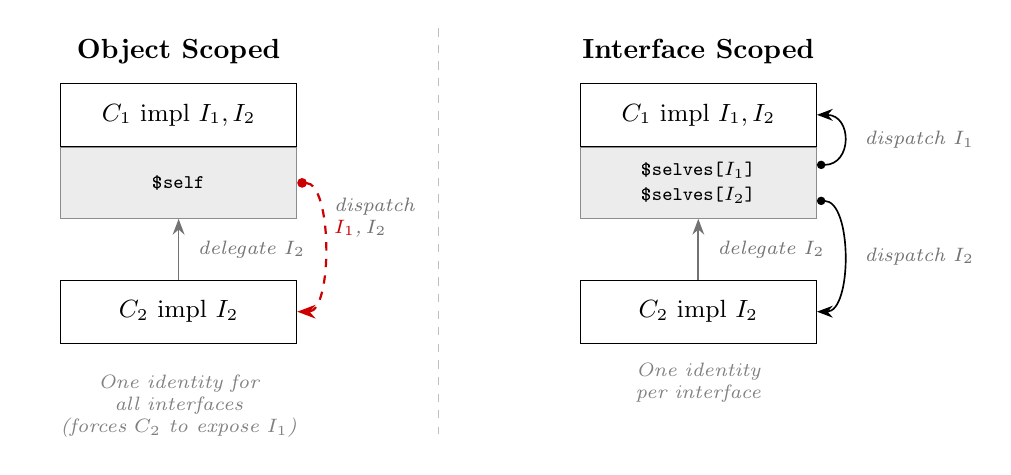
\begin{tikzpicture}[
  >=Stealth,
  cbox/.style={draw, rectangle, minimum width=3cm, minimum height=0.8cm,
               inner sep=5pt, align=center, font=\small},
  % Both bars share the same minimum height so C1+bar is equal width on both sides
  sbar/.style={draw=black!45, fill=gray!15, rectangle,
               minimum width=3cm, minimum height=0.9cm,
               inner sep=3pt, align=right, font=\scriptsize\ttfamily},
  svbar/.style={draw=black!45, fill=gray!15, rectangle,
                minimum width=3cm, minimum height=0.9cm,
                inner sep=3pt, align=right, font=\scriptsize\ttfamily},
  darr/.style={->, black!55, semithick},
]

%%---- Left panel (Object Scoped) -----------------------------------
\node[font=\bfseries] at (-3.3, 3.3) {Object Scoped};

\node[cbox] (TopL) at (-3.3, 2.5) {$C_1$ impl $I_1$,\,$I_2$};
\node[sbar, below=0pt of TopL] (BarL) {\texttt{\$self}};
\node[cbox] (BotL) at (-3.3, 0.0) {$C_2$ impl $I_2$};

\coordinate (midL) at ($(BarL.south)!0.5!(BotL.north)$);

\draw[darr] (BotL.north) -- (BarL.south);
\node[font=\scriptsize\itshape, text=black!55, anchor=west]
  at ($(midL -| BotL.north) + (0.12, 0)$) {delegate $I_2$};

% $self arc: single composite identity dispatches all interfaces
\draw[{Circle[fill=red!80!black,scale=0.7]}->, red!80!black, thick, dashed]
  (BarL.east)
  .. controls ($(BarL.east)+(0.45,0)$) and ($(BotL.east)+(0.45,0)$) ..
  (BotL.east)
  node[pos=0.5, anchor=south west, font=\scriptsize\itshape, text=black!55,
       align=left] {dispatch\\\textcolor{red!80!black}{$I_1$},\,$I_2$};

%%---- Divider -------------------------------------------------------
\draw[black!25, dashed] (0, 3.6) -- (0, -1.55);

%%---- Right panel (Interface Scoped) --------------------------------
\node[font=\bfseries] at (3.3, 3.3) {Interface Scoped};

\node[cbox] (TopR) at (3.3, 2.5) {$C_1$ impl $I_1$,\,$I_2$};
\node[svbar, below=0pt of TopR] (BarR)
  {\texttt{\$selves[$I_1$]}\\[1pt]\texttt{\$selves[$I_2$]}};
\node[cbox] (BotR) at (3.3, 0.0) {$C_2$ impl $I_2$};

\coordinate (midR) at ($(BarR.south)!0.5!(BotR.north)$);

\draw[darr] (BotR.north) -- (BarR.south);
\node[font=\scriptsize\itshape, text=black!55, anchor=west]
  at ($(midR -| BotR.north) + (0.12, 0)$) {delegate $I_2$};

% Named exit points on $selves bar
\coordinate (selI1) at ($(BarR.north east)!0.25!(BarR.south east)$);
\coordinate (selI2) at ($(BarR.north east)!0.75!(BarR.south east)$);

% $selves[I1] → TopR: I1 scoped identity dispatches to C1
\draw[{Circle[fill=black,scale=0.7]}->, semithick]
  (selI1)
  .. controls ($(selI1)+(0.45,0)$) and ($(TopR.east)+(0.45,0)$) ..
  (TopR.east)
  node[pos=0.5, anchor=west, xshift=4pt, font=\scriptsize\itshape,
       text=black!55] {dispatch $I_1$};

% $selves[I2] → BotR: I2 scoped identity dispatches to C2
\draw[{Circle[fill=black,scale=0.7]}->, semithick]
  (selI2)
  .. controls ($(selI2)+(0.45,0)$) and ($(BotR.east)+(0.45,0)$) ..
  (BotR.east)
  node[pos=0.5, anchor=west, xshift=4pt, font=\scriptsize\itshape,
       text=black!55] {dispatch $I_2$};

%%---- Panel captions -----------------------------------------------
\node[font=\scriptsize\itshape, text=black!50,
      text width=3.6cm, align=center] at (-3.3,-1.2)
  {One identity for all interfaces\\(forces $C_2$ to expose $I_1$)};
\node[font=\scriptsize\itshape, text=black!50,
      text width=3cm, align=center] at (3.3,-0.9)
  {One identity per interface};

\end{tikzpicture}
\caption{Object-scoped vs.\ interface-scoped dispatch. In both panels $C_2$
(impl~$I_2$) delegates $I_2$ to $C_1$ (impl~$I_1$,\,$I_2$).
\emph{Left:} \texttt{\$self} holds the full composite identity; a self-call
$m() \in I_1$ inside $C_1$ routes through \texttt{\$self\,=\,$C_2$}, the outer
composite, requiring $C_2$ to implement $I_1$ to avoid a cast
failure, a constraint $C_2$ may not satisfy.
\emph{Right:} each \texttt{\$selves[$I_i$]} slot holds a scoped identity;
$m() \in I_1$ dispatches through \texttt{\$selves[$I_1$]}, routing directly
to $C_1$ without involving $C_2$; $n() \in I_2$ dispatches through
\texttt{\$selves[$I_2$]}, routing to $C_2$.}
\label{fig:dispatch-comparison}
\end{figure}

\begin{proposition}
\label{prop:dispatch}
For any component $P$ in a delegation chain for interface $I$ rooted at
composite $C$: a self-call \code{this.m()} within $P$ where $m \in I$
dispatches to $C$.
\end{proposition}

The invariant is established by construction. When composite $C$ establishes
a link to component $P$ for interface $I$, the plugin-generated
\code{\$linkPartToSelf} sets $\$\mathit{selves}_P[I] \leftarrow C$ and
recurses into $P$'s own links, propagating $C$'s identity for each interface
$C$ claims and leaving all other slots unchanged. Each interface of a component resolves
through a single \code{\$selves} slot. Wiring an outer composite that claims
$I$ re-roots this slot to that composite and leaves the slots for interfaces it
does not claim unchanged, so the slot holds exactly one root at any time and
stabilizes once the outermost composite claiming $I$ is wired; $C$ denotes that
final root. Each write occurs during the wiring composite's construction. Link
fields are \code{final} (enforced by the plugin); once the composition rooted at
$C$ is safely published, the Java Memory Model guarantees any thread that
observes $C$ sees the fully wired \code{\$selves} slots, which are not written
thereafter. Self-calls in $P$ where $m \in I$ are rewritten by
the plugin to \code{((I)\,\$selves[IDX\_I]).m()}; when $m$ belongs to multiple
interfaces (the diamond case), $I$ is determined at compile time by diamond
resolution (Section~\ref{sec:impl}). For self-calls through the delegation surface, there is no code path in a
\code{@part} method that dispatches through anything other than the indexed
slot. Because the slot holds $C$ once the composition is constructed and is not
written thereafter, the invariant holds at every point a self-call can execute.
Before wiring, each slot is initialized to \code{this}; an unwired component
dispatches on itself, consistent with standard object-oriented dispatch, and
the Proposition is vacuously satisfied (no delegation chain exists).
A full mechanized proof in a Featherweight Java subset is a natural direction
for follow-on work (Section~\ref{sec:futurework}).

%% ─────────────────────────────────────────────────────────────────────────────
\section{Implementation}
\label{sec:impl}
%% ─────────────────────────────────────────────────────────────────────────────

The implementation is a \texttt{javac} plugin operating on the compiler's AST
during two phases. In \textsc{enter}, the plugin generates structural
scaffolding: the \code{\$selves} composite identity array and
\code{\$linkPartToSelf} wiring method for each \code{@part} class, delegation
method skeletons for each composite class, and (for abstract components) the
\code{\$Impl} subclass and \code{asLink()} factories. In \textsc{analyze},
after type resolution, self-calls in \code{@part} bodies are rewritten,
\code{@link} field assignments are rewritten to invoke wiring, and
\code{@internal} visibility is enforced. No bytecode manipulation is performed;
all transformation is at the AST level and subject to standard type checking.

\subsection{Component Transformation}

Each \code{@part} class holds a \code{\$selves} array indexed by interface
ordinal, assigned at compile time:

\begin{lstlisting}[language={},style=java]
private final Object[] $selves = {this, ..., this};
// after wiring: $selves[IDX_I] = composite identity for interface I
\end{lstlisting}

An unwired component dispatches on itself; once wired, dispatch routes through
the composite identity. \code{\$linkPartToSelf} updates each relevant slot and
recurses through \code{@link} fields in the component whose delegation surface
includes the interface being propagated, leaving all other slots unchanged, with
cycle detection at each assignment.

\subsection{Rewriting}

Within a \code{@part} method body, every call \code{this.m(args)} where
\code{m} is declared in interface $I$ is rewritten to:

\begin{lstlisting}
((I) $selves[IDX_I]).m(args)
\end{lstlisting}

The cast to $I$ selects the dispatch interface explicitly; when diamond
resolution has assigned $m$ to a specific authoritative link, $I$ is that
link's interface, determined at compile time.

A composite implements every interface claimed by its links. For each method of
a claimed interface that the composite does not declare itself, the plugin
generates a delegating method that forwards through the corresponding
\code{@link} field:

\begin{lstlisting}
R m(args) { return link.m(args); }   // void methods omit the return
\end{lstlisting}

A method the composite declares itself is left as written, and no forwarder is
generated for it. When two links share an interface, the forwarders for the
shared methods route through the authoritative link
(Definition~\ref{def:diamond}). The forwarder is a plain forward; routing a
component's self-call back to the composite is handled by that component's
\code{\$selves} slot (above), not by the forwarder.

In composite classes, each \code{@link} field assignment \code{this.link = expr}
is rewritten to invoke \code{\$linkPartToSelf}, propagating the composite
identity into the component. An \code{instanceof} check guards the call so
that non-\code{@part} assignments pass through unchanged.

\subsection{Abstract Component Support}

A \code{@part} class may be abstract, deferring some interface methods to the
composite. Linking an abstract part obligates the composite to implement those
methods or to be declared abstract, enforced at compile time: the plugin
generates a delegating method for every interface method the part implements and
none for a method it leaves abstract, so a concrete composite is missing exactly
those methods and \texttt{javac} rejects it unless they are supplied directly.
This is the compositional analog of the rule that a concrete class must implement
its inherited abstract methods.

To make an abstract part instantiable for linking, the compiler generates a
private \code{\$Impl} subclass whose stubs throw \code{DelegationLinkageError},
and an \code{asLink()} factory per non-private constructor:

\begin{lstlisting}
private static final class $Impl extends Foo {
    $Impl(/* Foo constructor params */) { super(/* Foo constructor params */); }
    @Override public T m(Params p) {
        throw new DelegationLinkageError("abstract method called on an unlinked part");
    }
}
public static Foo asLink(/* Foo constructor params */) { return new $Impl(/* same */); }
\end{lstlisting}

Once wired, the stubs are unreachable: self-calls dispatch through
\code{\$selves[IDX\_I]} to the composite, whose implementation the compile-time
obligation guarantees. The stubs remain only as a runtime guard for an
\code{asLink()} instance invoked before it is wired.

\subsection{Default Methods}

A default method's body is declared in the interface, not in a \code{@part}, so
the self-call rewrite of Section~\ref{sec:impl} never sees its self-calls.
Invoked on a wired component, an inherited default would run with \code{this}
bound to the component, and its self-calls would resolve within the component
rather than through the composite.

For a default method a component does not override, the plugin generates a
forwarder that routes on wiring state. Unwired, it runs the interface default
directly (\code{I.super.m()}, \code{this} the component); this is the standalone
case. Wired, it invokes the interface's default \emph{implementation} with the
composite as receiver, so the default body's self-calls dispatch through the
composite. A default the component overrides needs no such forwarder: the
override is an ordinary \code{@part} method whose self-calls are rewritten
through \code{\$selves} like any other. An explicit \code{I.super.m()} written
in component code is rewritten to the same composite-rooted invocation.

Invoking a default body on a chosen receiver has no plain-bytecode form (no
instruction invokes an interface default on an object other than the current
receiver), so the wired reroute compiles to an \code{invokedynamic} call site.
Its bootstrap method resolves, once per site at linkage, a handle that invokes
the interface's default body with the composite as receiver, and returns a
constant call site. The target is fixed (the interface's default body); only the
receiver varies, as a call argument. The site is therefore monomorphic, and once
linked the JIT treats the handle as a constant and inlines the default body into
the caller: dispatch on par with the array-indexed \code{invokeinterface} of
Section~\ref{sec:eval}. The only addition over the concrete-method path is the
forwarder's wiring-state test, a single branch on the \code{final}
\code{\$selves} slot that resolves one way once the composition is constructed.
The decorator and
template-method patterns of Section~\ref{sec:eval} stay O(1) whether their
template is written as a concrete \code{@part} method or as an interface default.

\subsection{\code{@internal} Enforcement}

\code{@internal} may annotate an interface method or an interface type literal
in a class's \code{implements} clause, with distinct effects. An interface
method marked \code{@internal} is not accessible to code external to the
composite; calls from outside the composite are compile errors, while calls
via \code{@link} field references within the composite are permitted. An
interface type literal marked \code{@internal} in a class's \code{implements}
clause removes that interface from the class's delegation surface: no external
composite may claim it via a \code{@link} field.

\subsection{Safety Guarantees}

\paragraph{Cycle detection.}
If a component is wired to itself directly or transitively,
\code{De\-le\-ga\-tion\-Link\-age\-Er\-ror} is thrown at assignment time during
the recursive \code{\$linkPartToSelf()} call.

\paragraph{Deferred method access.}
The obligation that a wired composite implement an abstract part's deferred
methods is enforced at compile time; the residual case is an \code{asLink()}
instance invoked before it is wired into any composite, where the \code{\$Impl}
stub throws \code{DelegationLinkageError}, the compositional analog of
\code{AbstractMethodError}.

\paragraph{Self-preservation.}
Inside a \code{@part}, \code{this} use is guarded. Field access, private calls,
and callbacks through the part's own \code{@link} fields (the compositional
analog of \code{super}) are all permitted. Passing or assigning \code{this} as
the concrete \code{@part} type is not: that is a compile error, since a caller
holding the bare component could invoke methods outside the composite dispatch
path and violate Proposition~\ref{prop:dispatch}. The only \code{this} that can
leave is therefore interface-typed, and the reference that crosses is the
\code{\$selves} slot for that interface: the component's composite identity for
it, which may be the component itself. A client receiving it reaches the
composite's overrides; recovering some other interface by reflection or
downcast can still reach a lower root (Section~\ref{sec:limitations}).

%% ─────────────────────────────────────────────────────────────────────────────
\section{Evaluation}
\label{sec:eval}
%% ─────────────────────────────────────────────────────────────────────────────

\subsection{Dispatch Performance}

The dispatch path for a self-call through a composite is:
\begin{enumerate}
  \item Load \code{\$selves[IDX\_I]}, an array-indexed load with compile-time
        constant index
  \item Cast to $I$
  \item \code{invokeinterface m}, standard JVM virtual dispatch
\end{enumerate}

This is O(1). The parallel to vtable dispatch is direct: a vtable
call is an indexed slot load followed by an indirect call. Call sites in typical
compositions are monomorphic or bimorphic, the JIT's most aggressively optimized
scenarios. Composite dispatch adds at most one additional virtual dispatch over
direct delegation.

\paragraph{Benchmark.}
We verify this empirically using JMH~\cite{jmh} in average-time mode.
Each scenario calls \code{compute()} through a composite root at chain
depth $d$ (1--6). The \emph{baseline} traverses $d$ \code{@link} delegation
hops to a leaf that returns directly, with no self-call; the \emph{ISD}
variant traverses the same hops but the leaf issues a self-call
(\code{\$selves[IDX\_I].scale()}), dispatching through the composite root.
The delta between the two isolates the cost of the self-call dispatch
mechanism alone, independent of delegation depth. All runs: 3 JVM forks,
5 warmup iterations, 10 measurement iterations per fork (30 data points per
cell); errors are $\pm$\,half-width of the 99.9\% confidence interval.
A separate single-dispatch calibration run (\code{invokeinterface}
on a monomorphic call site, same harness) yields 0.46\,ns/op; the delta
values in Table~\ref{tab:bench} are therefore roughly 1--2$\times$ a single virtual
dispatch.

\begin{table}[H]
\centering
\caption{Self-call dispatch cost by delegation depth (JMH, average-time mode; ns/op, $\pm$\,99.9\% CI half-width). The delta isolates the cost of the self-call dispatch over plain delegation. All values are rounded from unrounded measurements; the delta and its interval are computed from the unrounded statistics, so the delta may differ from the rounded baseline/ISD difference by~0.01\,ns.}
\label{tab:bench}
{\small
\begin{tabular}{crrr}
\toprule
Depth & Baseline (ns) & ISD (ns) & Delta (ns) \\
\midrule
1 & $0.65 \pm 0.03$ & $1.24 \pm 0.03$ & $0.59 \pm 0.04$ \\
2 & $0.93 \pm 0.05$ & $1.65 \pm 0.05$ & $0.71 \pm 0.07$ \\
3 & $1.25 \pm 0.05$ & $2.05 \pm 0.07$ & $0.81 \pm 0.09$ \\
4 & $1.67 \pm 0.02$ & $2.43 \pm 0.10$ & $0.76 \pm 0.10$ \\
5 & $2.12 \pm 0.05$ & $2.91 \pm 0.05$ & $0.79 \pm 0.07$ \\
6 & $2.52 \pm 0.11$ & $3.46 \pm 0.11$ & $0.94 \pm 0.16$ \\
\bottomrule
\end{tabular}
}
\end{table}

\noindent
The delta is stable across depths (0.6--0.8\,ns at depths 1--5, 0.94\,ns at depth 6), with overlapping
confidence intervals at depths 2--5. At sub-nanosecond resolution,
microbenchmark variance makes fine-grained trend analysis unreliable;
the O(1) argument is structural; the stable delta band corroborates it. The delta is
consistent with one array-indexed load (\code{\$selves[IDX\_I]}) followed by
\code{invokeinterface}.

\subsection{Example: Teaching Assistant}

The following example exercises DAG composition, diamond dispatch resolution,
and self-call routing through the composite. A teaching assistant is both
a student and a teacher; both roles share a common \code{Person} base.

\begin{lstlisting}
interface Person  { String getName(); String getTitle(); String getTitledName(); }
interface Student extends Person { String getMajor(); }
interface Teacher extends Person { String getDept();   }
interface TA      extends Student, Teacher {}
\end{lstlisting}

\paragraph{Forwarding~\cite{kotlin,lombok}.}
Forwarding-based mechanisms inject the implementation as a real object at
construction time; components are independent. But self-calls remain within
the component: the composite is invisible. Delegating
\code{Student by s} and \code{Teacher by t} creates a diamond: the compiler
forces a manual override of every shared \code{Person} method. The deeper problem is that
\code{getTitledName()}---the template method worth sharing---cannot be safely
delegated: whichever branch receives it calls \code{getTitle()} on its own
\code{this}, bypassing \code{TaImpl.getTitle()}.

\begin{lstlisting}[style=kotlin]
class TaImpl(val s: Student, val t: Teacher) : TA,
    Student by s, Teacher by t {
  // Diamond: every shared Person method must be manually resolved
  override fun getName()  = s.getName()
  override fun getTitle() = "TA"
  // Without this override, getTitledName() forwards to s.getTitledName(),
  // which calls s.getTitle() = "Student" -- self stays in the delegate:
  //   TaImpl(...).getTitledName()  ->  "Student Milton"  (wrong)
  override fun getTitledName() = "${getTitle()} ${getName()}"
  //   TaImpl(...).getTitledName()  ->  "TA Milton"       (correct, but forced)
}
\end{lstlisting}

Every composite must re-implement \code{getTitledName()}.
Adding a new template method to \code{Person} requires a matching override in
every composite class; the maintenance cost grows with the number of composites. Lombok's
\code{@Delegate} generates equivalent forwarders in Java; the self-call
semantics are identical.

\paragraph{Parts.}
\code{PersonPart} holds the template once. Its self-call to \code{getTitle()}
dispatches through the composite at each level of the delegation chain.

\begin{lstlisting}
@part class PersonPart implements Person {
  private final String name;
  public PersonPart(String name) { this.name = name; }
  public String getName()       { return name; }
  public String getTitle()      { return "Person"; }
  public String getTitledName() { return getTitle() + " " + getName(); }
}
@part class StudentPart implements Student {
  @link Person person;
  private final String major;
  public StudentPart(Person p, String major) { this.person = p; this.major = major; }
  public String getTitle()  { return "Student"; }
  public String getMajor()  { return major; }
}
@part class TeacherPart implements Teacher {
  @link Person person;
  private final String dept;
  public TeacherPart(Person p, String dept) { this.person = p; this.dept = dept; }
  public String getTitle() { return "Teacher"; }
  public String getDept()  { return dept; }
}
@part class TaPart implements TA {
  @link(share=Person.class) Student student;
  @link Teacher teacher;
  public TaPart(Student s) {
    this.student = s;
    this.teacher = new TeacherPart(s, "Math");
  }
  public String getTitle() { return "TA"; }
}

TA ta = new TaPart(new StudentPart(new PersonPart("Milton"), "CS"));
ta.getTitledName(); // "TA Milton"  -- getTitle() dispatches through TaPart
\end{lstlisting}

\code{getTitledName()} is defined once in \code{PersonPart} and overridden
nowhere. Diamond resolution is handled statically: \code{@link(share=Person.class)}
designates \code{student} as the authoritative delegate for \code{Person},
so \code{Person} is excluded from propagation when \code{teacher} is wired,
leaving the identity established through \code{student} intact.

\subsection{Case Study: Stream Decoration}

A pattern common in the JDK---exemplified by \code{java.io.InputStream}~\cite{gamma1994}---is
a bulk operation implemented as a loop over a finer one: \code{read(byte[],
int, int)} calls the single-byte \code{read()} repeatedly. Decorators override
\code{read()} to add behavior; the template is supposed to propagate it to bulk
calls automatically. The \code{Readable} interface below captures this contract
directly. Under forwarding, the propagation breaks.

A \code{CountingStream} that tracks bytes consumed overrides \code{read()} to
increment a counter. With Lombok's \code{@Delegate}, \code{read(byte[], int, int)} is
forwarded to the delegate, which calls \code{read()} on itself, not on
\code{CountingStream}. The override is never reached for bulk calls.

\paragraph{Forwarding~\cite{lombok}.}

\begin{lstlisting}
interface Readable {
    int read();
    int read(byte[] buf, int off, int len);
}

class BaseStream implements Readable {
    private final byte[] data;
    private int pos;
    BaseStream(byte[] data) { this.data = data; }
    public int read() { return pos < data.length ? (data[pos++] & 0xff) : -1; }
    public int read(byte[] buf, int off, int len) {
        for (int i = 0; i < len; i++) {
            int b = read();                      // self-call
            if (b == -1) return i == 0 ? -1 : i;
            buf[off + i] = (byte) b;
        }
        return len;
    }
}

class CountingStream implements Readable {
    @Delegate private final Readable delegate;
    private int count;
    CountingStream(Readable r) { this.delegate = r; }
    @Override public int read() {
        int b = delegate.read();
        if (b != -1) count++;
        return b;
    }
    public int count() { return count; }
}

CountingStream cs = new CountingStream(new BaseStream(data));
cs.read(buf, 0, 16);  // -> delegate.read(byte[],int,int)
                       //    -> delegate.read()  -- not cs.read()
cs.count();            // 0  -- bulk reads not counted
\end{lstlisting}

\paragraph{Parts.}
\code{BaseStream} is unchanged except for the \code{@part} annotation. The
self-call in \code{read(byte[], int, int)} routes through \code{CountingStream}
on every call path.

\begin{lstlisting}
@part class BaseStream implements Readable { /* same as above */ }

class CountingStream implements Readable {
    @link Readable stream;
    private int count;
    CountingStream(Readable r) { this.stream = r; }
    @Override public int read() {
        int b = stream.read();
        if (b != -1) count++;
        return b;
    }
    public int count() { return count; }
}

CountingStream cs = new CountingStream(new BaseStream(data));
cs.read(buf, 0, 16);  // -> BaseStream.read(byte[],int,int)
                       //    -> self-call read() -> CountingStream.read()
cs.count();            // 16  -- all bytes counted
\end{lstlisting}

A new decorator---buffering, decryption, rate limiting---requires only
overriding \code{read()}; \code{BaseStream.read(byte[], int, int)} routes its
self-call through whichever composite is the dispatch root, without
modification.

\subsection{Test Coverage}

The implementation is tested against a suite covering:
\begin{itemize}
  \item forwarding vs.\ delegation semantics
  \item DAG composition at depth $\geq 3$
  \item diamond detection and resolution
  \item abstract component / \code{asLink()} lifecycle
  \item \code{@internal} interface and method enforcement
  \item default method dispatch
  \item inheritance chains in \code{@part} hierarchies
  \item cycle detection (runtime \code{DelegationLinkageError})
\end{itemize}

\subsection{Limitations}\label{sec:limitations}

\begin{itemize}
  \item Using \code{@link}, \code{@part}, and \code{@internal} requires
        configuring the \texttt{javac} plugin in the build system (Maven,
        Gradle, or similar).
  \item Composite dispatch semantics are not enforced against runtime
        introspection that reaches past a reference's supplied static type. A
        client that reflects on an escaped reference, or downcasts it to an
        interface it was not handed, can invoke that interface below its
        composite root, bypassing the overrides above it; type-directed
        clients, which use the interface they were handed, are unaffected.
        This is by design.
  \item The plugin relies on internal \texttt{javac} APIs for AST
        rewriting.
\end{itemize}

%% ─────────────────────────────────────────────────────────────────────────────
\section{Discussion}
\label{sec:discussion}
%% ─────────────────────────────────────────────────────────────────────────────

\subsection{Implementation Identity and Dispatch Identity}

A composition model that supports independent components must handle two
structural scenarios:

\begin{itemize}
  \item \textbf{Partial delegation}: a composite delegates a subset of a
        component's interfaces.
  \item \textbf{Multi-root}: a component's interfaces are claimed by separate
        composites, each requiring a distinct dispatch root from the same
        instance.
\end{itemize}

Multi-root requires a component to carry multiple simultaneous
composite identities, one per interface. ISD resolves this by separating \emph{implementation identity} (the
component object) from \emph{dispatch identity} (the composite per
interface). Within ISD, partial delegation and multi-root are modeled the same way. Every
interface has a single composition receiver: the composite that claims it, or the
component itself when none does.

Multi-root arises naturally from partial delegation: when an outer composite claims a subset of a
component's interfaces, transitive propagation assigns different roots to the
remaining interfaces, producing multi-root at the component level. The \code{Track} example in
Section~\ref{sec:model} demonstrates this directly: \code{Library} claims
only \code{Classifiable} from \code{Playlist} (partial delegation), which by propagation
gives \code{Track} separate roots for \code{Streamable} and
\code{Classifiable} (multi-root).

\subsection{Language Design Implications}

Extending any statically-typed OO language with a composition model equivalent
to \code{@link}\allowbreak/\code{@part} would satisfy both properties. The model addresses
each failure mode that has kept implementation inheritance in use:

\begin{itemize}
  \item \textbf{Fragile base class}~\cite{mikhajlov1998}: a composite's dependency surface is
        the interface contracts it explicitly claims, not a component's internal
        implementation; changes to its encapsulated internals do not propagate. Partial
        delegation completes the isolation: a composite is unaffected by changes
        to interfaces it did not claim.
  \item \textbf{Forced IS-A semantics}: reuse does not require a type
        relationship; the composite IS-A the interface, not the component.
  \item \textbf{The Self problem}: a hazard in forwarding-based composition
        where self-calls remain within the component rather than routing
        through the composite; resolved by ISD.
  \item \textbf{Diamond ambiguity}: explicit \code{@link(share=T.class)} resolution;
        unresolved diamonds are compile errors, not silent merges.
  \item \textbf{Encapsulation breach}: a composite may implement a subset
        of its parts' interfaces; those it does not implement are absent from
        its API by construction. \code{@internal} strengthens this further:
        it provides composite-scoped visibility, preventing designated
        interfaces from being delegated by any external composite.
  \item \textbf{Abstract behavior}: abstract components with deferred
        linkage (\code{asLink()}) preserve the template-method capability
        of abstract classes without coupling the hierarchy.
\end{itemize}

Underlying these is one shift. Implementation inheritance's power is open
recursion: a base method's self-calls reach the most-derived overrides. Its
fragility is the surface that recursion ranges over: every overridable method
and protected member. Parts keeps the open recursion but bounds it to the
declared interface; self-calls still reach the composite's overrides, while the
encapsulated internals that make base classes fragile stay off the recursion
entirely.

Interface inheritance, which provides type contracts and is foundational
to this model, is untouched. The same choice that keeps the delegation surface
a contract---interfaces rather than implementation types---is what makes
dispatch constant-time: a fixed, statically-known interface set lets each
interface's root be an array-indexed slot. The self-preservation constraint---that a
\code{@part} class may not expose \code{this} as its concrete type---is
not a limitation but the static guarantee that makes the dispatch invariant
hold.

Implementation inheritance and Parts are two bindings of the same open
recursion: implementation inheritance binds it to the class hierarchy, where a
subclass IS-A its superclass and inherits its entire implementation surface,
while Parts binds it to a held object and a declared interface, where the
composite HAS-A its components and IS-A only their interfaces. That inheritance
is open recursion, separable from subtyping, is
Cook's~\cite{cookpalsberg1989,cook1990}, and the reading of inheritance as
composition is Bracha and Cook's~\cite{bracha1990}; the missing piece has been a
realization with independent runtime components, static interface contracts, and
dispatch at the cost of a virtual call.

\subsection{Concurrency}

The DAG structure is favorable for concurrent use. Component wiring occurs
during construction; once the composition is fully constructed and its root
safely published, the JMM guarantees all wired \code{\$selves} state is visible
to any thread that observes the root. The slots are not written after
construction; no synchronization is required for dispatch.
Components may contain mutable state, subject to the usual Java concurrency
rules; the dispatch mechanism adds no additional synchronization points.

\subsection{Future Work}
\label{sec:futurework}

\paragraph{Formal verification.}
A full mechanized proof of Proposition~\ref{prop:dispatch} in a small-step operational semantics
would provide assurance beyond the construction argument above. The model maps
cleanly to a subset of Featherweight Java, a natural starting point for that formalization.

\paragraph{Per-interface composite roots as a general primitive.}
The structural insight underlying this model---that dispatch identity can be
assigned per interface rather than per object---opens a solution space that
prior single-composite-identity models cannot reach. Problems currently addressed
suboptimally through dynamic dispatch, AOP weaving, or collapsed component
hierarchies may admit statically sound solutions within this primitive.

%% ─────────────────────────────────────────────────────────────────────────────
\section{Related Work}
\label{sec:related}
%% ─────────────────────────────────────────────────────────────────────────────

Static typing is the baseline requirement; models without it are included where
they complete the landscape.

\paragraph{Forwarding.}
Kotlin's \code{by} keyword~\cite{kotlin} generates forwarding methods at compile
time; Lombok's \code{@Delegate}~\cite{lombok} does the same in Java; Scala~3's
\code{export} keyword~\cite{scala3export} generates forwarding methods for
delegated members.
In all cases, a component's self-calls resolve within the component; the composite
host is invisible. The mechanism is forwarding, not delegation. Scala
provides both mechanisms in the same language: \code{export}
for forwarding with independent components, and traits for correct self-call
dispatch. Yet no combination of the two satisfies both requirements.
B\"uchi and Weck's generic wrappers~\cite{buchi2000} give the same forwarding
choice a formal, soundness-proven treatment, and are the closest prior analysis of
the identity-escape hazard our self-preservation constraint prevents
(Section~\ref{sec:impl}), though they decline the disciplines we adopt as too
restrictive for arbitrary legacy objects.

\paragraph{Scala traits / abstract type members.}
Odersky and Zenger~\cite{odersky2005} introduced statically-typed mixin
composition with abstract type members. Scala's \code{with} clause linearizes
traits into the target class at compile time. Self-calls dispatch through the
outermost class in the linearized hierarchy. Linearization also fuses the
component into the class hierarchy: trait implementations are resolved at
compile time and cannot be supplied as late-bound objects at construction. A composite that holds its own implementation of one interface while delegating
another from the same component requires independent component objects, which
linearization precludes.

\paragraph{Prototype-based delegation.}
Lieberman~\cite{lieberman1986} introduced \emph{open delegation}: an object may
delegate unanswered messages to a prototype, with \emph{self} remaining the
original receiver throughout the chain. Self~\cite{self1987} realized this in a
working language. These systems support correct self-call dispatch with late-bound
components in arbitrary delegation graphs. Static type guarantees are absent by
design.

\paragraph{Mixins.}
Bracha and Cook~\cite{bracha1990} formalized mixins as parameterized abstract
subclasses. Mixins extend through linearization: the mixin is applied to a chain at class
definition time, not supplied as a late-bound object at construction.
Self-calls dispatch through \code{this} in the linearized result.

\paragraph{Traits.}
Sch\"arli et al.~\cite{scharli2003} proposed traits as stateless, composable
units of behavior. Trait composition is a compile-time operation: methods are
flattened into the target class, not supplied as late-bound objects at
construction. Self-calls dispatch through \code{this} in the composed class.

\paragraph{Multiple inheritance.}
Stroustrup~\cite{stroustrup1987} introduced virtual base classes and virtual
inheritance in C++ to handle diamonds. The result is a single linearized object
with a merged vtable; components are not preserved as independent objects.

\paragraph{Kniesel / Lava.}
Kniesel's ``type-safe delegation''~\cite{kniesel1999,kniesel2000} shares this
paper's goal most closely: components are real runtime objects supplied at
construction, types are statically enforced, and DARWIN binds \texttt{self} to
the original receiver so self-calls route through the composite rather than
staying in the component. The realized cost is not constant. DARWIN compiles to
per-message parent casts and forwarding adapters; by Kniesel's own analysis the
adapters ``accumulate in front of the adapted objects,'' and the typical
configuration (an abstract or interface parent type with a concrete subtype
instance, the same case \code{@link} targets) ``can be slowed down
significantly''~\cite[\S7.4]{kniesel2000}. The proposed remedies either double
every method (``weak customization,'' whose payoff Kniesel calls
``questionable'') or defer to the JIT a cost elimination that ``remains to be
evaluated''~\cite[\S7.5]{kniesel2000}; the system was realized only in Lava, a
research language. Kniesel dismissed the static alternative of storing identity
in the component on two grounds: ``sharing of one parent by multiple delegating
children cannot be expressed at all,'' and recursive delegation could be
simulated only ``with significant run-time and software maintenance
costs''~\cite{kniesel1999}. Interface-scoped dispatch reopens that route on both
counts: indexing the stored identity by interface gives multiple composites
claiming disjoint interfaces of a shared component each its own root, and
transitive propagation wires recursive delegation chains at construction, so
dispatch stays constant-time and the chain adds no per-call cost or maintenance
burden.

\paragraph{Delegation Layers.}
Ostermann's delegation layers~\cite{ostermann2002} (ECOOP 2002) combine
delegation with virtual classes to compose collaborations dynamically at
runtime; self-calls route correctly within a composed collaboration. The unit
composed is the collaboration (a layer of virtual nested classes bound to a
common enclosing type), not the individual object; participants are members of
that collaboration, not components supplied independently per interface.

\paragraph{Virtual classes and family polymorphism.}
The virtual-class lineage (gbeta~\cite{ernst2001}, CaesarJ~\cite{aracic2006},
Object Teams/Java~\cite{herrmann2002}, and J\&~\cite{nystrom2006}) achieves open class composition through virtual nested
classes within a common enclosing family type; Ernst, Ostermann, and
Cook~\cite{ernst2006} provide the definitive formal treatment.
Components are runtime instances of virtual classes, but they are bound to an
enclosing family type and cannot be independently supplied from outside.
Self-calls dispatch correctly within the family.

\paragraph{Dynamic composition.}
Newspeak~\cite{bracha2010} treats classes as first-class late-bound arguments,
enabling runtime composition of first-class module objects with correct
self-call dispatch. Static type checking is absent by design.

%% ─────────────────────────────────────────────────────────────────────────────
\section{Conclusion}
%% ─────────────────────────────────────────────────────────────────────────────

Forwarding-based composition supplies independent components but not self-call dispatch: calls through \texttt{this} resolve within
the component, not through the composite. Trait and mixin composition
preserves self-call dispatch but not independent components; composition is
static, linearized into the class hierarchy at compile time. No prior
statically-typed approach delivers both at the cost of ordinary dispatch.

Interface-scoped dispatch resolves both. Assigning composite identity per
interface rather than per object gives each self-call a well-defined route
through the correct composite, at the cost of one array-indexed load plus
standard \texttt{invokeinterface}, structurally equivalent to vtable dispatch.
The cost holds even in the general case, where components with multiple
composite roots arise by structural necessity from ordinary partial delegation.

The Self problem with independent components has gone without a practical
solution since 1986. It is a large part of why object composition never displaced
implementation inheritance: a self-call
that reaches the composite's overrides is the one capability that made
inheritance necessary rather than merely convenient. ISD closes that gap.


%% ─────────────────────────────────────────────────────────────────────────────
%% References
%% ─────────────────────────────────────────────────────────────────────────────

\begin{thebibliography}{10}

\bibitem{gamma1994}
E.~Gamma, R.~Helm, R.~Johnson, and J.~Vlissides.
\newblock {\em Design Patterns: Elements of Reusable Object-Oriented Software}.
\newblock Addison-Wesley, 1994.

\bibitem{mikhajlov1998}
L.~Mikhajlov and E.~Sekerinski.
\newblock A study of the fragile base class problem.
\newblock In {\em Proceedings of ECOOP}, LNCS 1445, pages 355--382, 1998.

\bibitem{lieberman1986}
H.~Lieberman.
\newblock Using prototypical objects to implement shared behavior in
  object-oriented systems.
\newblock In {\em Proceedings of OOPSLA}, pages 214--223, 1986.

\bibitem{bracha1990}
G.~Bracha and W.~Cook.
\newblock Mixin-based inheritance.
\newblock In {\em Proceedings of OOPSLA/ECOOP}, pages 303--311, 1990.

\bibitem{cookpalsberg1989}
W.~Cook and J.~Palsberg.
\newblock A denotational semantics of inheritance and its correctness.
\newblock In {\em Proceedings of OOPSLA}, pages 433--443, 1989.

\bibitem{cook1990}
W.~R.~Cook, W.~Hill, and P.~S.~Canning.
\newblock Inheritance is not subtyping.
\newblock In {\em Conference Record of POPL}, pages 125--135, 1990.

\bibitem{scharli2003}
N.~Sch{\"a}rli, S.~Ducasse, O.~Nierstrasz, and A.~Black.
\newblock Traits: Composable units of behaviour.
\newblock In {\em Proceedings of ECOOP}, LNCS 2743, pages 248--274, 2003.

\bibitem{self1987}
D.~Ungar and R.~B.~Smith.
\newblock Self: The power of simplicity.
\newblock In {\em Proceedings of OOPSLA}, pages 227--242, 1987.

\bibitem{odersky2005}
M.~Odersky and M.~Zenger.
\newblock Scalable component abstractions.
\newblock In {\em Proceedings of OOPSLA}, pages 41--57, 2005.

\bibitem{stroustrup1987}
B.~Stroustrup.
\newblock Multiple inheritance for {C++}.
\newblock In {\em Proceedings of the EUUG Spring Conference}, 1987.

\bibitem{kniesel1999}
G.~Kniesel.
\newblock Type-safe delegation for run-time component adaptation.
\newblock In {\em Proceedings of ECOOP}, LNCS 1628, pages 351--366, 1999.
\newblock DOI: \href{https://doi.org/10.1007/3-540-48743-3_16}{10.1007/3-540-48743-3\_16}.

\bibitem{kniesel2000}
G.~Kniesel.
\newblock {\em Dynamic Object-Based Inheritance with Subtyping}.
\newblock PhD thesis, University of Bonn, 2000.

\bibitem{buchi2000}
M.~B\"uchi and W.~Weck.
\newblock Generic wrappers.
\newblock In {\em Proceedings of ECOOP}, LNCS 1850, pages 201--225, 2000.

\bibitem{ostermann2002}
K.~Ostermann.
\newblock Dynamically composable collaborations with delegation layers.
\newblock In {\em Proceedings of ECOOP}, LNCS 2374, pages 89--110, 2002.

\bibitem{ernst2006}
E.~Ernst, K.~Ostermann, and W.~R.~Cook.
\newblock A virtual class calculus.
\newblock In {\em Conference Record of POPL}, pages 270--282, 2006.

\bibitem{nystrom2006}
N.~Nystrom, X.~Qi, and A.~C.~Myers.
\newblock {J\&}: Nested intersection for scalable software composition.
\newblock In {\em Proceedings of OOPSLA}, pages 347--366, 2006.

\bibitem{ernst2001}
E.~Ernst.
\newblock Family polymorphism.
\newblock In {\em Proceedings of ECOOP}, LNCS 2072, pages 303--326, 2001.

\bibitem{aracic2006}
I.~Aracic, V.~Gasiunas, M.~Mezini, and K.~Ostermann.
\newblock An overview of {CaesarJ}.
\newblock In {\em Transactions on Aspect-Oriented Software Development I}, LNCS 3880, pages 135--173, 2006.

\bibitem{herrmann2002}
S.~Herrmann.
\newblock Object {Teams}: Improving modularity for crosscutting collaborations.
\newblock In {\em Proceedings of NetObjectDays}, LNCS 2591, pages 248--264, 2002.

\bibitem{bracha2010}
G.~Bracha, P.~von~der~Ah{\'e}, V.~Bykov, Y.~Kashai, W.~Maddox, and E.~Miranda.
\newblock Modules as objects in {Newspeak}.
\newblock In {\em Proceedings of ECOOP}, LNCS 6183, pages 405--428, 2010.

\bibitem{scala3export}
EPFL.
\newblock Exports --- {Scala~3} reference.
\newblock \url{https://docs.scala-lang.org/scala3/reference/other-new-features/export.html}, 2024.

\bibitem{kotlin}
JetBrains.
\newblock Delegation --- {Kotlin} programming language.
\newblock \url{https://kotlinlang.org/docs/delegation.html}, 2024.

\bibitem{lombok}
Project Lombok.
\newblock \texttt{@Delegate} --- {Lombok} features.
\newblock \url{https://projectlombok.org/features/Delegate}, 2024.

\bibitem{jmh}
A.~Shipilev and contributors.
\newblock {JMH}: Java Microbenchmark Harness.
\newblock \url{https://github.com/openjdk/jmh}, 2013--2024.

\bibitem{mckinney2026}
R.~S.~McKinney.
\newblock manifold-delegation.
\newblock \url{https://github.com/manifold-systems/manifold/tree/master/manifold-deps-parent/manifold-delegation}, 2026.

\end{thebibliography}





\end{document}
